\documentclass[12pt,a4paper]{report}

% Encoding and Fonts
\usepackage[utf8]{inputenc}
\usepackage[T1]{fontenc}
\usepackage{times}

% Packages for Mathematics and Symbols
\usepackage{amsmath, amsfonts, amssymb}
\usepackage{bm}

% Packages for Graphics and Figures
\usepackage{graphicx}
\usepackage{float}
\usepackage{tikz}
\usetikzlibrary{arrows.meta, positioning, shapes.multipart, calc}
\usepackage{pgfgantt}
\usepackage{caption}
\usepackage{subcaption}

% Packages for Hyperlinks
\usepackage{hyperref}
\hypersetup{
    colorlinks=true,
    linkcolor=blue,
    urlcolor=blue,
    citecolor=blue
}

% Page Layout
\usepackage{geometry}
\geometry{a4paper, margin=1in}

% Header and Footer
\usepackage{fancyhdr}
\pagestyle{fancy}
\fancyhf{}
\setlength{\headheight}{26.98592pt}
\fancyhead[L]{\leftmark}
\fancyfoot[C]{\thepage}

% Section Formatting
\usepackage{titlesec}
\titleformat{\chapter}[display]
  {\normalfont\huge\bfseries\color{blue}}
  {\chaptername\ \thechapter}{20pt}{\Huge}
\titlespacing*{\chapter}{0pt}{0pt}{20pt}

% Table of Contents Formatting
\usepackage{tocloft}
\renewcommand{\cftchapfont}{\bfseries}
\renewcommand{\cftsecfont}{\bfseries}

% Bibliography
\usepackage{cite}

% Package for Algorithms
\usepackage{algorithm}
\usepackage{algorithmic}

% Package for Multirow in Tables
\usepackage{multirow}

% Package for Adjusting Table Columns
\usepackage{array}

% Line Spacing
\usepackage{setspace}
\onehalfspacing % 1.5 spacing

% Document Information
\title{\textbf{Hybrid Data Augmentation Techniques for Disease Identification from Clinical Notes}}
\author{
    \textbf{Kaustabh Ganguly} \\
    Roll Number: CH23M514 \\
    \\
    \textbf{Mentors}: \\
    Samyabrata Chakraborty \\
    Debopam Nanda \\
}
\date{November 30, 2024}

\begin{document}

% Cover Page
\begin{titlepage}
    \centering
    
\includegraphics[width=4cm]{logo.png} \\
    \vspace{0.5cm}
    {\large \bfseries M.Tech Project Report\\
    INDIAN INSTITUTE OF TECHNOLOGY MADRAS \\
    CHENNAI -- 600036} \\
    \vspace{1.5cm}
    {\huge \bfseries Hybrid Data Augmentation Techniques for Disease Identification from Clinical Notes} \\
    \vspace{2cm}
    {\Large \textit{A Project Report}} \\
    \vspace{0.5cm}
    {\large Submitted by} \\
    \vspace{0.5cm}
    {\Large \bfseries Kaustabh Ganguly} \\
    \vspace{0.5cm}
    {\large For the award of the degree of} \\
    \vspace{0.5cm}
    {\Large \bfseries MASTER OF TECHNOLOGY} \\
    \vspace{1.5cm}
    {\large \bfseries November 2024} \\
    \vfill
    {\small \textcopyright~2024 Indian Institute of Technology Madras}
\end{titlepage}

% Thesis Certificate Page
\newpage
~\vfill
\begin{center}
    \textbf{Thesis Certificate}
\end{center}
\vspace{0.5in}
This is to certify that the thesis titled \textit{``Hybrid Data Augmentation Techniques for Disease Identification from Clinical Notes''} submitted by \textbf{Kaustabh Ganguly}, Roll Number \textbf{CH23M514}, is a bona fide record of the work done under our guidance. \\

\vspace{1in}

\noindent \textbf{Mentors}: \\
Samyabrata Chakraborty \hfill Signature: \\
Debopam Nanda \hfill Signature: \\

\vfill
\newpage

% Abstract
\chapter*{Abstract}
Accurately assigning \textbf{International Classification of Diseases (ICD)} codes to clinical narratives is essential for efficient healthcare operations, research, and patient care. However, this task is challenging, particularly for \textbf{rare diseases}, due to the scarcity of annotated clinical notes and data imbalance. This thesis addresses the problem of predicting ICD codes from clinical narratives, specifically focusing on improving accuracy for rare codes.

Adopting a design thinking approach, we identified the needs of healthcare professionals and the limitations of existing systems. We propose a method that utilizes \textbf{Retrieval Augmented Generation (RAG)} to create synthetic clinical notes for rare diseases. By connecting RAG with medical knowledge bases, we generate realistic clinical narratives that augment the \textbf{MIMIC-IV} dataset, enriching the data available for rare ICD codes. This augmentation aims to balance the dataset and enhance the learning process of predictive models.

In the initial phase, we established a robust development environment, implemented data version control, and explored extensive medical datasets and knowledge graphs. Preliminary experiments with traditional machine learning models highlighted significant challenges due to data imbalance and the complexity of clinical texts. Specifically, our baseline models struggled to predict rare ICD codes, confirming the impact of data imbalance on model performance and reinforcing the necessity for advanced techniques.

Our ongoing work involves integrating RAG with medical knowledge to generate synthetic data and employing transformer-based deep learning models to predict ICD codes. By augmenting the dataset with diverse clinical narratives, we anticipate a significant improvement in prediction accuracy for rare ICD codes.

This research contributes to the field by addressing data scarcity in medical coding through innovative data augmentation techniques. The outcomes aim to enhance automated ICD coding systems, reduce the burden on healthcare professionals, and ultimately support better healthcare delivery.

% Table of Contents
\tableofcontents
\newpage

% Chapters

\chapter{Introduction}

\section{Background}
Accurate medical coding is essential in modern healthcare systems for various purposes, including billing, epidemiology, research, and clinical decision support. The \textbf{International Classification of Diseases (ICD)} is a standardized system developed by the World Health Organization (WHO) for coding diseases, symptoms, and procedures~\cite{who2019icd11}. In particular, the latest version, \textbf{ICD-11}, provides a comprehensive coding system used globally.

\section{Importance of ICD Coding}
ICD codes serve as a critical link between clinical care and administrative functions. They are used for:
\begin{itemize}
    \item \textbf{Billing and Reimbursement}: Accurate coding ensures that healthcare providers are appropriately reimbursed for the services provided.
    \item \textbf{Clinical Research}: Researchers use ICD codes to identify patient populations and study disease prevalence and outcomes.
    \item \textbf{Public Health Surveillance}: Health authorities monitor disease outbreaks and trends using aggregated ICD code data.
    \item \textbf{Healthcare Planning}: Policy-makers rely on coding data to allocate resources and plan healthcare services.
\end{itemize}

\section{Challenges in Manual ICD Coding}
Despite its importance, manual ICD coding is a complex and time-consuming process. Trained medical coders must interpret unstructured clinical narratives and assign appropriate codes. Challenges include:
\begin{itemize}
    \item \textbf{Volume of Data}: Healthcare facilities generate vast amounts of clinical documentation daily.
    \item \textbf{Complexity of Coding Systems}: The ICD system contains thousands of codes, with ICD-10-CM having around 68,000 diagnosis codes~\cite{dong2022automated}.
    \item \textbf{Ambiguity in Clinical Language}: Clinical notes often contain ambiguous or colloquial language, making interpretation difficult.
    \item \textbf{Human Error}: Manual coding is prone to errors, which can lead to incorrect billing, compliance issues, and compromised data quality.
\end{itemize}

\section{Need for Automated ICD Coding}
To address these challenges, there is a pressing need for automated ICD coding systems that can:
\begin{itemize}
    \item \textbf{Improve Efficiency}: Reduce the time and effort required for manual coding.
    \item \textbf{Enhance Accuracy}: Minimize human errors and improve coding consistency.
    \item \textbf{Support Scalability}: Handle large volumes of clinical data efficiently.
    \item \textbf{Facilitate Data Utilization}: Enable better use of clinical data for research and decision-making.
\end{itemize}

\section{Challenges in Automated ICD Coding}
While automated ICD coding holds promise, it faces several significant challenges:
\begin{itemize}
    \item \textbf{Data Imbalance and Scarcity}: Clinical datasets exhibit a long-tailed distribution of ICD codes, with a few codes being highly frequent and many codes occurring rarely~\cite{rios2018few}. Models often perform poorly on rare codes due to insufficient training data.
    \item \textbf{Complexity of Clinical Texts}: Clinical narratives are lengthy, unstructured, and contain domain-specific terminology, abbreviations, and inconsistencies~\cite{wrenn2010quantifying}.
    \item \textbf{Multi-Label Classification}: Assigning ICD codes is a multi-label task, where multiple codes may be relevant for a single clinical note.
    \item \textbf{Explainability and Interpretability}: Healthcare professionals require transparent and interpretable models to trust and adopt automated coding systems~\cite{holzinger2017we}.
\end{itemize}

\section{Existing Approaches and Limitations}
Various machine learning and deep learning approaches have been proposed for automated ICD coding:
\begin{itemize}
    \item \textbf{Rule-Based Systems}: Early methods relied on handcrafted rules and keyword matching but lacked scalability and adaptability~\cite{farkas2008automatic}.
    \item \textbf{Traditional Machine Learning}: Techniques like Support Vector Machines and Decision Trees were used but struggled with high-dimensional, sparse data and failed to capture semantic nuances~\cite{perotte2014diagnosis}.
    \item \textbf{Deep Learning Models}: Convolutional Neural Networks (CNNs) and Recurrent Neural Networks (RNNs) have improved performance by learning hierarchical representations of text~\cite{mullenbach2018explainable, vu2020label}. However, they often underperform on rare codes due to data imbalance.
    \item \textbf{Transformer-Based Models}: Models like BERT have advanced natural language understanding but may not consistently outperform CNNs in clinical text classification and face challenges with long documents~\cite{dong2022automated, gao2021limitations}.
    \item \textbf{Curriculum Learning and Hierarchical Models}: Methods like HiCu leverage the hierarchical structure of ICD codes to improve performance on rare codes~\cite{ren2022hicu}.
\end{itemize}

Despite these advancements, significant gaps remain in effectively handling data imbalance, processing complex clinical texts, and providing explainable predictions.

\section{Problem Statement}
In this thesis, we address the problem of accurately predicting ICD codes from clinical narratives, with a focus on improving performance on rare codes. The key challenges include:
\begin{itemize}
    \item \textbf{Data Imbalance}: Handling the long-tailed distribution of ICD codes and the scarcity of annotated data for rare codes.
    \item \textbf{Complexity of Clinical Texts}: Processing lengthy and unstructured clinical narratives to extract relevant information.
    \item \textbf{Explainability}: Providing interpretable predictions to gain clinician trust.
\end{itemize}

\section{Proposed Solution}
To tackle these challenges, we propose a comprehensive approach that includes:
\begin{itemize}
    \item \textbf{Hybrid Data Augmentation}: Combining Retrieval Augmented Generation (RAG) with ontology-based methods to generate synthetic clinical notes for rare diseases, augmenting the training data.
    \item \textbf{Knowledge Integration}: Leveraging medical ontologies and knowledge graphs (e.g., SNOMED CT, RxNorm) to enrich data representation and model understanding of medical concepts.
    \item \textbf{Transformer-Based Models}: Utilizing advanced transformer architectures adapted for long clinical documents to capture contextual information.
    \item \textbf{Multi-Label Classification Techniques}: Implementing label embedding, hierarchical classification, and label grouping to handle the extensive label space.
    \item \textbf{Explainability Techniques}: Integrating methods like SHAP, LIME, and Integrated Gradients to provide transparent insights into model predictions.
\end{itemize}

\section{Objectives}
The objectives of this thesis are:
\begin{enumerate}
    \item Develop an advanced, explainable model for ICD code prediction, focusing on rare codes.
    \item Implement hybrid data augmentation techniques to address data imbalance.
    \item Integrate medical knowledge through ontologies and knowledge graphs.
    \item Enhance model interpretability to facilitate clinical acceptance.
\end{enumerate}

\section{Thesis Outline}
The remainder of this thesis is organized as follows.
\begin{itemize}
    \item \textbf{Chapter 2: Literature Review} – A detailed review of existing approaches and challenges in automated ICD coding.
    \item \textbf{Chapter 3: Definition and formulation of the problem} – A precise statement of the problem and its formulation.
    \item \textbf{Chapter 4: Methodology} – An in-depth explanation of the proposed methods and details of the implementation.
    \item \textbf{Chapter 5: Dataset Understanding} – A description of the datasets used and their characteristics.
    \item \textbf{Chapter 6: Results} – Presentation and analysis of the experimental results.
    \item \textbf{Chapter 7: Conclusion and Work Timeline} – A summary of the work and the plan for completing the remaining tasks.
\end{itemize}

\chapter{Literature Review}

The automation of the International Classification of Diseases (ICD) coding process has emerged as a critical area of research in medical informatics and Natural Language Processing (NLP). The ICD is a globally recognized system used for classifying diseases and health conditions, essential for epidemiological studies, health management, and clinical billing. Manual ICD coding involves assigning appropriate codes to clinical narratives, a task that is both time-consuming and prone to errors due to the complexity and volume of medical records. The transition from ICD-9 to ICD-10 and now to ICD-11 has further increased the complexity, with a significant expansion in the number of codes and granularity~\cite{who2019icd11}.

\section{Early Approaches to Automated ICD Coding}

Early approaches to automate ICD coding primarily relied on rule-based systems and traditional machine learning techniques. Rule-based methods utilized handcrafted rules, regular expressions, and keyword matching to map clinical terms to ICD codes~\cite{farkas2008automatic, scheurwegs2017data}. While these approaches achieved high precision in specific contexts, they lacked scalability and adaptability to the extensive and evolving ICD code sets. The complexity and dynamic nature of classification systems, such as ICD-10-CM with around 68,000 diagnosis codes~\cite{dong2022automated}, posed significant challenges for rule-based systems to cover all possible coding scenarios.

Traditional machine learning methods, such as Support Vector Machines (SVMs) and Decision Trees, employed feature engineering to represent clinical texts numerically~\cite{perotte2014diagnosis}. These methods often required extensive preprocessing and could not effectively capture the semantic richness of clinical narratives. Moreover, they struggled with high-dimensional and sparse data characteristic of clinical texts and did not generalize well to unseen or rare codes.

\section{Deep Learning in Automated ICD Coding}

The advent of deep learning has revolutionized NLP by enabling models to learn hierarchical and abstract representations of text data without extensive feature engineering~\cite{lecun2015deep}. In the context of automated ICD coding, deep learning models have been employed to effectively capture complex patterns in clinical narratives and improve coding accuracy.

\subsection{Convolutional and Recurrent Neural Networks}

Convolutional Neural Networks (CNNs) have been applied to capture local syntactic and semantic patterns in text~\cite{kim2014convolutional}. Mullenbach et al.~\cite{mullenbach2018explainable} introduced the Convolutional Attention for Multi-Label classification (CAML) model, which employs a convolutional encoder followed by a label-wise attention mechanism. The attention mechanism allows the model to focus on relevant parts of the text for each ICD code, enhancing interpretability. The attention weights for each label $l$ are computed as:

\begin{equation}
\alpha^{(l)} = \text{softmax}(W^{(l)} h + b^{(l)}),
\end{equation}

where $h$ represents the hidden representations from the convolutional layers, and $W^{(l)}$, $b^{(l)}$ are the label-specific parameters.

Building upon CAML, Li and Yu~\cite{li2020multi} proposed the Multi-Filter Residual Convolutional Neural Network (MultiResCNN), which integrates residual connections and multiple convolutional filters to capture patterns at various granularities. The model enhances feature extraction and improves performance on the ICD coding task.

Recurrent Neural Networks (RNNs), particularly Long Short-Term Memory (LSTM) networks, have been utilized to capture sequential dependencies in clinical texts~\cite{hochreiter1997long}. Vu et al.~\cite{vu2020label} introduced the Label-Attention model (LAAT), which employs a bidirectional LSTM encoder and a structured self-attention mechanism to generate label-specific document representations. The attention mechanism in LAAT is formulated as:

\begin{equation}
A = \text{softmax}(U \tanh(P H)),
\end{equation}

where $H$ is the sequence of hidden states from the bidirectional LSTM, $P$ is a projection matrix, and $U$ is a label embedding matrix. The label-specific representations are then used to predict the ICD codes.

While these models have shown improvements over traditional methods, they still face limitations. CNNs, for instance, may not effectively capture long-range dependencies due to their local receptive fields. RNNs can model sequences but suffer from issues like vanishing gradients and computational inefficiency with long texts. Additionally, both CNNs and RNNs may struggle with the extensive label space and data imbalance inherent in ICD coding tasks.

\subsection{Transformer-Based Models}

Transformer-based models, such as BERT~\cite{devlin2019bert}, have further advanced the field by enabling models to capture long-range dependencies and contextual information through self-attention mechanisms. Huang et al.~\cite{huang2022plm} proposed the PLM-ICD model, which leverages pre-trained language models for the ICD coding task. The PLM-ICD model integrates a pre-trained BERT encoder with a label attention mechanism, allowing it to benefit from large-scale language pre-training and focus on relevant text segments for each code.

However, an empirical observation is that current BERT-based approaches do not consistently achieve better performance than CNN-based methods for multi-label classification applied to clinical coding~\cite{dong2022automated, gao2021limitations}. This limitation may be attributed to the inefficiency of BERT in modeling concept-level information and handling long clinical documents. Gao et al.~\cite{gao2021limitations} highlighted that BERT's fixed input length and computational complexity make it less suitable for processing lengthy discharge summaries without truncation, potentially leading to information loss.

Heo et al.~\cite{heo2022medical} addressed the challenge of applying BERT to long clinical documents by introducing the Document-to-Sequence BERT (D2SBERT) model. D2SBERT divides lengthy discharge summaries into multiple sequences of fixed length and processes each sequence independently using BERT. They then apply a sequence attention mechanism to capture important information across these sequences for ICD code prediction. Their experiments on the MIMIC-III dataset demonstrated that D2SBERT outperforms previous models, including CNN-based methods, in predicting ICD codes.

Despite these advances, transformer-based models still face challenges with data imbalance and the extensive ICD code label space. They often require large amounts of data to generalize well, which is problematic for rare codes with limited training examples.

\subsection{Curriculum Learning and Hierarchical Models}

Curriculum learning is a training strategy where models are exposed to training examples in a meaningful order, generally from easy to hard, to improve learning efficiency and performance~\cite{bengio2009curriculum}. In the context of automated ICD coding, the hierarchical structure of ICD codes presents an opportunity to apply curriculum learning by leveraging the relationships among codes.

Ren et al.~\cite{ren2022hicu} introduced Hierarchical Curriculum Learning (HiCu), an algorithm that utilizes the hierarchical structure of ICD codes to create a curriculum for multi-label classification models. HiCu constructs a label tree from the ICD code hierarchy and trains the model in a sequence of rounds, each focusing on a different level of the hierarchy. At each round, the model learns to predict codes at a particular level before proceeding to more specific codes in the next level.

The HiCu algorithm employs a knowledge transfer mechanism using hyperbolic embeddings to initialize model parameters for each level based on the parameters from the previous level. This approach ensures that the model builds upon previously learned representations, facilitating the learning of more complex and specific codes.

By integrating curriculum learning with hierarchical knowledge, HiCu aims to improve model generalization, particularly for rare and less frequent codes. Their experiments on the MIMIC-III dataset showed that HiCu significantly improves predictive performance across different neural architectures, including CNNs, RNNs, and transformer-based models. The method resulted in higher macro-AUC and macro-F1 scores, indicating better performance on rare codes.

HiCu addresses the challenge of data imbalance by emphasizing the hierarchical relationships among labels and gradually increasing the difficulty of the learning task. This method demonstrates the potential of curriculum learning and hierarchical modeling in enhancing automated ICD coding systems.

\section{Challenges in Automated ICD Coding}

Despite these advancements, automated ICD coding faces several significant challenges, as detailed by Dong et al.~\cite{dong2022automated}, Edin et al.~\cite{edin2023automated}, and Nguyen et al.~\cite{nguyen2023mimic}.

\subsection{Data Imbalance and Scarcity}

One of the primary issues is data imbalance and scarcity, particularly for rare ICD codes. Clinical datasets exhibit a long-tailed distribution of codes, where a few codes are highly frequent, and many codes occur rarely. In the MIMIC-III dataset~\cite{johnson2016mimic}, for example, around 5,000 codes appear fewer than 10 times in the training data, and over 50\% of codes never appear~\cite{rios2018few}. This imbalance leads to models that perform well on frequent codes but poorly on rare ones. Handling unseen, infrequent, and imbalanced labels is a key problem for multi-label classification with many labels.

Edin et al.~\cite{edin2023automated} conducted a critical review and replicability study, finding that models underperform on rare codes due to weak configurations, poorly sampled train-test splits, and insufficient evaluation. They corrected the calculation of the macro F1-score, which had been sub-optimally computed in previous studies due to the inclusion of codes missing from the test set. Their revised evaluation doubled the macro F1-scores and provided a more accurate assessment of model performance on rare codes.

Nguyen et al.~\cite{nguyen2023mimic} highlighted that MIMIC-IV includes both ICD-9 and ICD-10 codes, with significantly more documents and unique labels compared to MIMIC-III. They discussed the challenges posed by the long-tailed distribution of ICD codes in MIMIC-IV, where the majority of codes are rare. By evaluating existing methods under more extreme conditions with longer-tailed distributions and a higher number of ICD codes, they provided a more comprehensive assessment of model performance.

Ren et al.~\cite{ren2022hicu} addressed data imbalance by leveraging the hierarchical structure of ICD codes in a curriculum learning framework. By training models to predict codes at different levels of the hierarchy sequentially, their HiCu algorithm improves performance on rare codes, as demonstrated by higher macro-AUC and macro-F1 scores.

\subsection{Processing Long and Complex Clinical Documents}

Clinical narratives, such as discharge summaries, can be lengthy and contain redundant or irrelevant information, often referred to as "note bloat"~\cite{wrenn2010quantifying}. Models may struggle to identify the relevant information for each code within such documents. However, Edin et al.~\cite{edin2023automated} conducted an error analysis and found that document length had only a negligible impact on overall model performance, suggesting that other factors, such as code frequency, play a more significant role.

Heo et al.~\cite{heo2022medical} proposed D2SBERT to address the challenge of processing long clinical documents. By dividing documents into manageable sequences and applying a sequence attention mechanism, D2SBERT effectively captures important information across the entire document without truncating it. This approach allows transformer-based models to handle long texts and improves ICD code prediction accuracy.

\subsection{Explainability and Interpretability}

Explainability and interpretability are crucial in healthcare applications, as clinicians need to understand the rationale behind model predictions to trust and effectively use automated systems~\cite{holzinger2017we}. While attention mechanisms provide some level of interpretability by highlighting relevant text segments, the highlighted texts mostly indicate associations instead of causality. Further studies are needed to evaluate the usefulness of highlights for clinical coders and to integrate more inherently explainable methods, such as incorporating symbolic representations of the coding steps with deep learning.

Edin et al.~\cite{edin2024unsupervised} proposed an unsupervised approach to achieve supervised-level explainability in healthcare records. They introduced adversarial robustness training to improve explanation plausibility and proposed a new explanation method, AttInGrad, which combines attention and gradient-based attributions. Their method produces explanations of comparable quality to supervised approaches without the need for costly evidence-span annotations.

Ren et al.~\cite{ren2022hicu} utilized hyperbolic embeddings and knowledge transfer mechanisms in their HiCu algorithm, which not only improves predictive performance but also provides insights into the hierarchical relationships among ICD codes. By structuring the learning process according to the ICD code hierarchy, their method enhances interpretability by aligning the model's learning trajectory with the established medical coding system.

\section{Embedding Models and Clinical Semantic Search}

The effectiveness of embedding models in medical semantic search tasks is critical for various applications, including document retrieval and information extraction. Excoffier et al.~\cite{excoffier2024generalist} compared generalist embedding models with specialized clinical embedding models in a semantic search task using rephrased ICD-10-CM code descriptions. Their results showed that generalist models performed better than clinical models, suggesting that specialized models may be more sensitive to small changes in input that confuse them.

The study highlighted that generalist models, trained on larger and more diverse datasets, may have a more robust language understanding, even in clinical contexts. This finding is significant because it challenges the assumption that domain-specific models always outperform generalist models in specialized tasks. It suggests that the training data's diversity and quantity play a crucial role in model robustness and performance.

Heo et al.~\cite{heo2022medical} demonstrated the effective use of BERT-based models in the clinical domain by adapting the model to handle long documents through sequence attention. Their approach shows that transformer-based models can be effectively applied to clinical text classification tasks when appropriately modified to address domain-specific challenges.

\section{Integrating Knowledge-Based Methods and Synthetic Data Generation}

To address the limitations of current deep learning approaches, integrating knowledge-based methods and symbolic reasoning has been proposed~\cite{dong2022automated}. Knowledge graphs and medical ontologies, such as SNOMED CT, RxNorm, and UMLS, can provide structured semantic information that enhances data representation and captures relationships between medical concepts.

Studies have explored embedding-based approaches to incorporate knowledge graphs into deep learning models~\cite{teng2020explainable, xie2019ehr}. For example, Teng et al.~\cite{teng2020explainable} utilized knowledge graphs to enhance the explainability and performance of ICD coding models by integrating semantic information from medical ontologies.

Ren et al.~\cite{ren2022hicu} employed hyperbolic embeddings to capture the hierarchical structure of ICD codes in their HiCu algorithm. Hyperbolic embeddings are effective in representing hierarchical data due to their ability to model tree-like structures in a continuous space with low distortion~\cite{nickel2017poincare}. By incorporating hyperbolic embeddings, HiCu leverages the ICD code hierarchy to improve model performance and interpretability.

Synthetic data generation has emerged as a promising approach to address data scarcity and imbalance in medical coding tasks. The generation of synthetic clinical notes can augment existing datasets, particularly for rare diseases, and enhance model performance.

Kumichev et al.~\cite{kumichev2024medsyn} introduced \textit{MedSyn}, a medical text generation framework that integrates large language models (LLMs) with a Medical Knowledge Graph (MKG). By sampling prior medical information from the MKG and generating synthetic clinical notes using GPT-4 and fine-tuned LLaMA models, they demonstrated that synthetic data could increase the classification accuracy of vital and challenging ICD codes by up to 17.8\% compared to settings without synthetic data.

\section{Summary of Literature Review}

Automated ICD coding is a promising application of AI in healthcare, offering potential improvements in efficiency and accuracy of the coding process. However, significant challenges remain, including handling data imbalance, processing long and complex documents, integrating symbolic reasoning, and ensuring explainability. Combining deep learning with knowledge-based methods, curriculum learning, and synthetic data generation, as well as involving clinical coders in the development process, are critical steps toward addressing these challenges.

Recent studies have emphasized the importance of innovative methodologies, standardized benchmarks, replicable experimental setups, and rigorous evaluation methods in automated ICD coding research. By addressing replicability issues, providing open-source code and data processing pipelines, and exploring novel data augmentation techniques, they facilitate fair comparisons and accelerate progress in the field.

Future research should focus on developing models that effectively integrate domain knowledge, handle rare and unseen codes, and provide transparent and explainable predictions. The integration of curriculum learning, advanced transformer models adapted for long clinical documents, and synthetic data generation holds promise for addressing data scarcity and enhancing model performance. Additionally, leveraging generalist embedding models in clinical tasks may improve robustness and effectiveness in semantic search applications. By addressing the technical and organizational challenges, automated clinical coding systems can be developed and deployed to support coding in the next five years and beyond.

\chapter{Problem Definition and Formulation}

\section{Problem Statement}
The primary goal of this research is to develop an automated system that accurately predicts \textbf{ICD codes} from unstructured \textbf{clinical narratives}, with a specific focus on improving prediction performance for \textbf{rare codes}.

\section{Challenges Addressed}
The problem encompasses several challenges:
\begin{itemize}
    \item \textbf{Data Imbalance}: The ICD code distribution is highly imbalanced, with rare codes having insufficient training examples.
    \item \textbf{Complexity of Clinical Texts}: Clinical narratives are lengthy, unstructured, and contain domain-specific language.
    \item \textbf{Multi-Label Classification}: Each clinical note may correspond to multiple ICD codes, requiring effective multi-label prediction.
    \item \textbf{Knowledge Integration}: Incorporating domain knowledge from medical ontologies to enhance model understanding.
    \item \textbf{Explainability}: Providing interpretable predictions to ensure clinical trust and acceptance.
\end{itemize}

\section{Problem Formulation}
Let \( D = \{(x_i, Y_i)\}_{i=1}^N \) denote the dataset, where \( x_i \) is the \( i \)-th clinical note and \( Y_i \subseteq \mathcal{L} \) is the set of ICD codes assigned to \( x_i \), with \( \mathcal{L} \) being the set of all ICD codes.

Our objective is to learn a function \( f: X \rightarrow 2^{\mathcal{L}} \) that maps a clinical note \( x \in X \) to a subset of ICD codes \( Y \subseteq \mathcal{L} \), such that \( f \) maximizes prediction accuracy, especially for rare codes.

\section{Handling Data Imbalance}
To address data imbalance, we aim to augment the dataset \( D \) by generating synthetic clinical notes \( \tilde{x}_j \) for rare ICD codes \( l \in \mathcal{L}_{\text{rare}} \), where \( \mathcal{L}_{\text{rare}} \subseteq \mathcal{L} \) denotes the set of rare codes. This involves creating a new set \( \tilde{D} = \{(\tilde{x}_j, Y_j)\} \) to supplement the original dataset, where \( Y_j \) includes rare codes.

\section{Knowledge Integration}
We seek to enrich the model's understanding by integrating knowledge from medical ontologies \( \mathcal{O} \) (e.g., SNOMED CT, RxNorm). This involves mapping clinical entities in \( x_i \) to concepts in \( \mathcal{O} \) and using this structured information in model training. Let \( \phi(x_i) \) denote the mapping from clinical notes to ontology concepts.

\section{Multi-Label Classification Approach}
Given the large label space and hierarchical relationships among ICD codes, we plan to employ advanced multi-label classification techniques:
\begin{itemize}
    \item \textbf{Label Embedding}: Representing ICD codes in a continuous space to capture semantic relationships.
    \item \textbf{Hierarchical Classification}: Leveraging the hierarchical structure of ICD codes to inform the classification process.
    \item \textbf{Label Grouping}: Grouping similar labels to reduce complexity and improve model efficiency.
\end{itemize}

\section{Evaluation Metrics}
To evaluate the performance of the model, especially on rare codes, we will use metrics that consider class imbalance:
\begin{itemize}
    \item \textbf{Macro F1-Score}: Calculated by averaging F1-scores across all labels, giving equal weight to rare and frequent codes.
    \item \textbf{F2-Score}: Emphasizes recall over precision, aligning with the need to reduce false negatives in medical coding.
\end{itemize}

\section{Specific Goals}
Our specific goals are:
\begin{enumerate}
    \item Achieve at least a 10\% improvement in macro F2-score on rare ICD codes compared to baseline models.
    \item Generate high-quality synthetic clinical notes for rare codes using hybrid data augmentation techniques.
    \item Integrate explainability methods to provide interpretable predictions acceptable to clinicians.
\end{enumerate}

\section{Constraints and Considerations}
\begin{itemize}
    \item \textbf{Data Privacy}: Ensure compliance with data use agreements and patient privacy regulations.
    \item \textbf{Computational Resources}: Optimize model design to work within available computational resources.
    \item \textbf{Clinical Relevance}: Engage with medical experts to validate the clinical plausibility of generated notes and model predictions.
\end{itemize}

\chapter{Methodology}

\section{Overview}
Our methodology involves several key components designed to address the challenges in automated ICD coding:
\begin{itemize}
    \item \textbf{Data Preparation and Exploration}
    \item \textbf{Hybrid Data Augmentation}
    \item \textbf{Transformer-Based Model Development}
    \item \textbf{Knowledge Integration}
    \item \textbf{Multi-Label Classification Techniques}
    \item \textbf{Model Training and Evaluation}
    \item \textbf{Explainability Integration}
\end{itemize}

\section{Data Preparation and Exploration}

\subsection{Development Environment Setup}
We established a robust development environment to facilitate efficient experimentation and model development:
\begin{itemize}
    \item \textbf{Version Control}: Implemented Data Version Control (DVC) for dataset tracking and management.
    \item \textbf{Model Tracking}: Utilized MLflow for tracking model experiments and parameters.
    \item \textbf{IDE Setup}: Configured VSCode and PyCharm for code development.
    \item \textbf{Database Tools}: Installed DataGrip and DBeaver for querying and managing databases.
\end{itemize}

\subsection{Data Storage and Processing}
To handle large datasets and enable efficient data processing:
\begin{itemize}
    \item \textbf{In-Memory Database}: Chose \textbf{DuckDB} for its ability to process data directly in memory with SQL queries, facilitating rapid data exploration.
    \item \textbf{Data Loading}: Loaded all 35 MIMIC-IV files into DuckDB, enabling SQL-based data manipulation.
\end{itemize}

\subsection{Data Exploration}
\begin{itemize}
    \item \textbf{Clinical Notes Extraction}: Focused on the \texttt{discharge.csv} file in MIMIC-IV Notes, containing discharge summaries.
    \item \textbf{ICD Code Association}: Joined clinical notes with \texttt{diagnoses\_icd.csv} using \texttt{hadm\_id} and \texttt{subject\_id} to associate notes with ICD codes.
    \item \textbf{Dataset Characteristics}: Identified that the dataset contains approximately 330,000 unique clinical notes and 40,000 patients, with a bias towards frequent ICD codes.
    \item \textbf{Data Distribution Analysis}: Analyzed the frequency distribution of ICD codes, confirming a long-tailed distribution where a small number of codes are highly frequent, and many are rare (Figure~\ref{fig:icd_distribution}).
\end{itemize}

\begin{figure}[H]
    \centering
    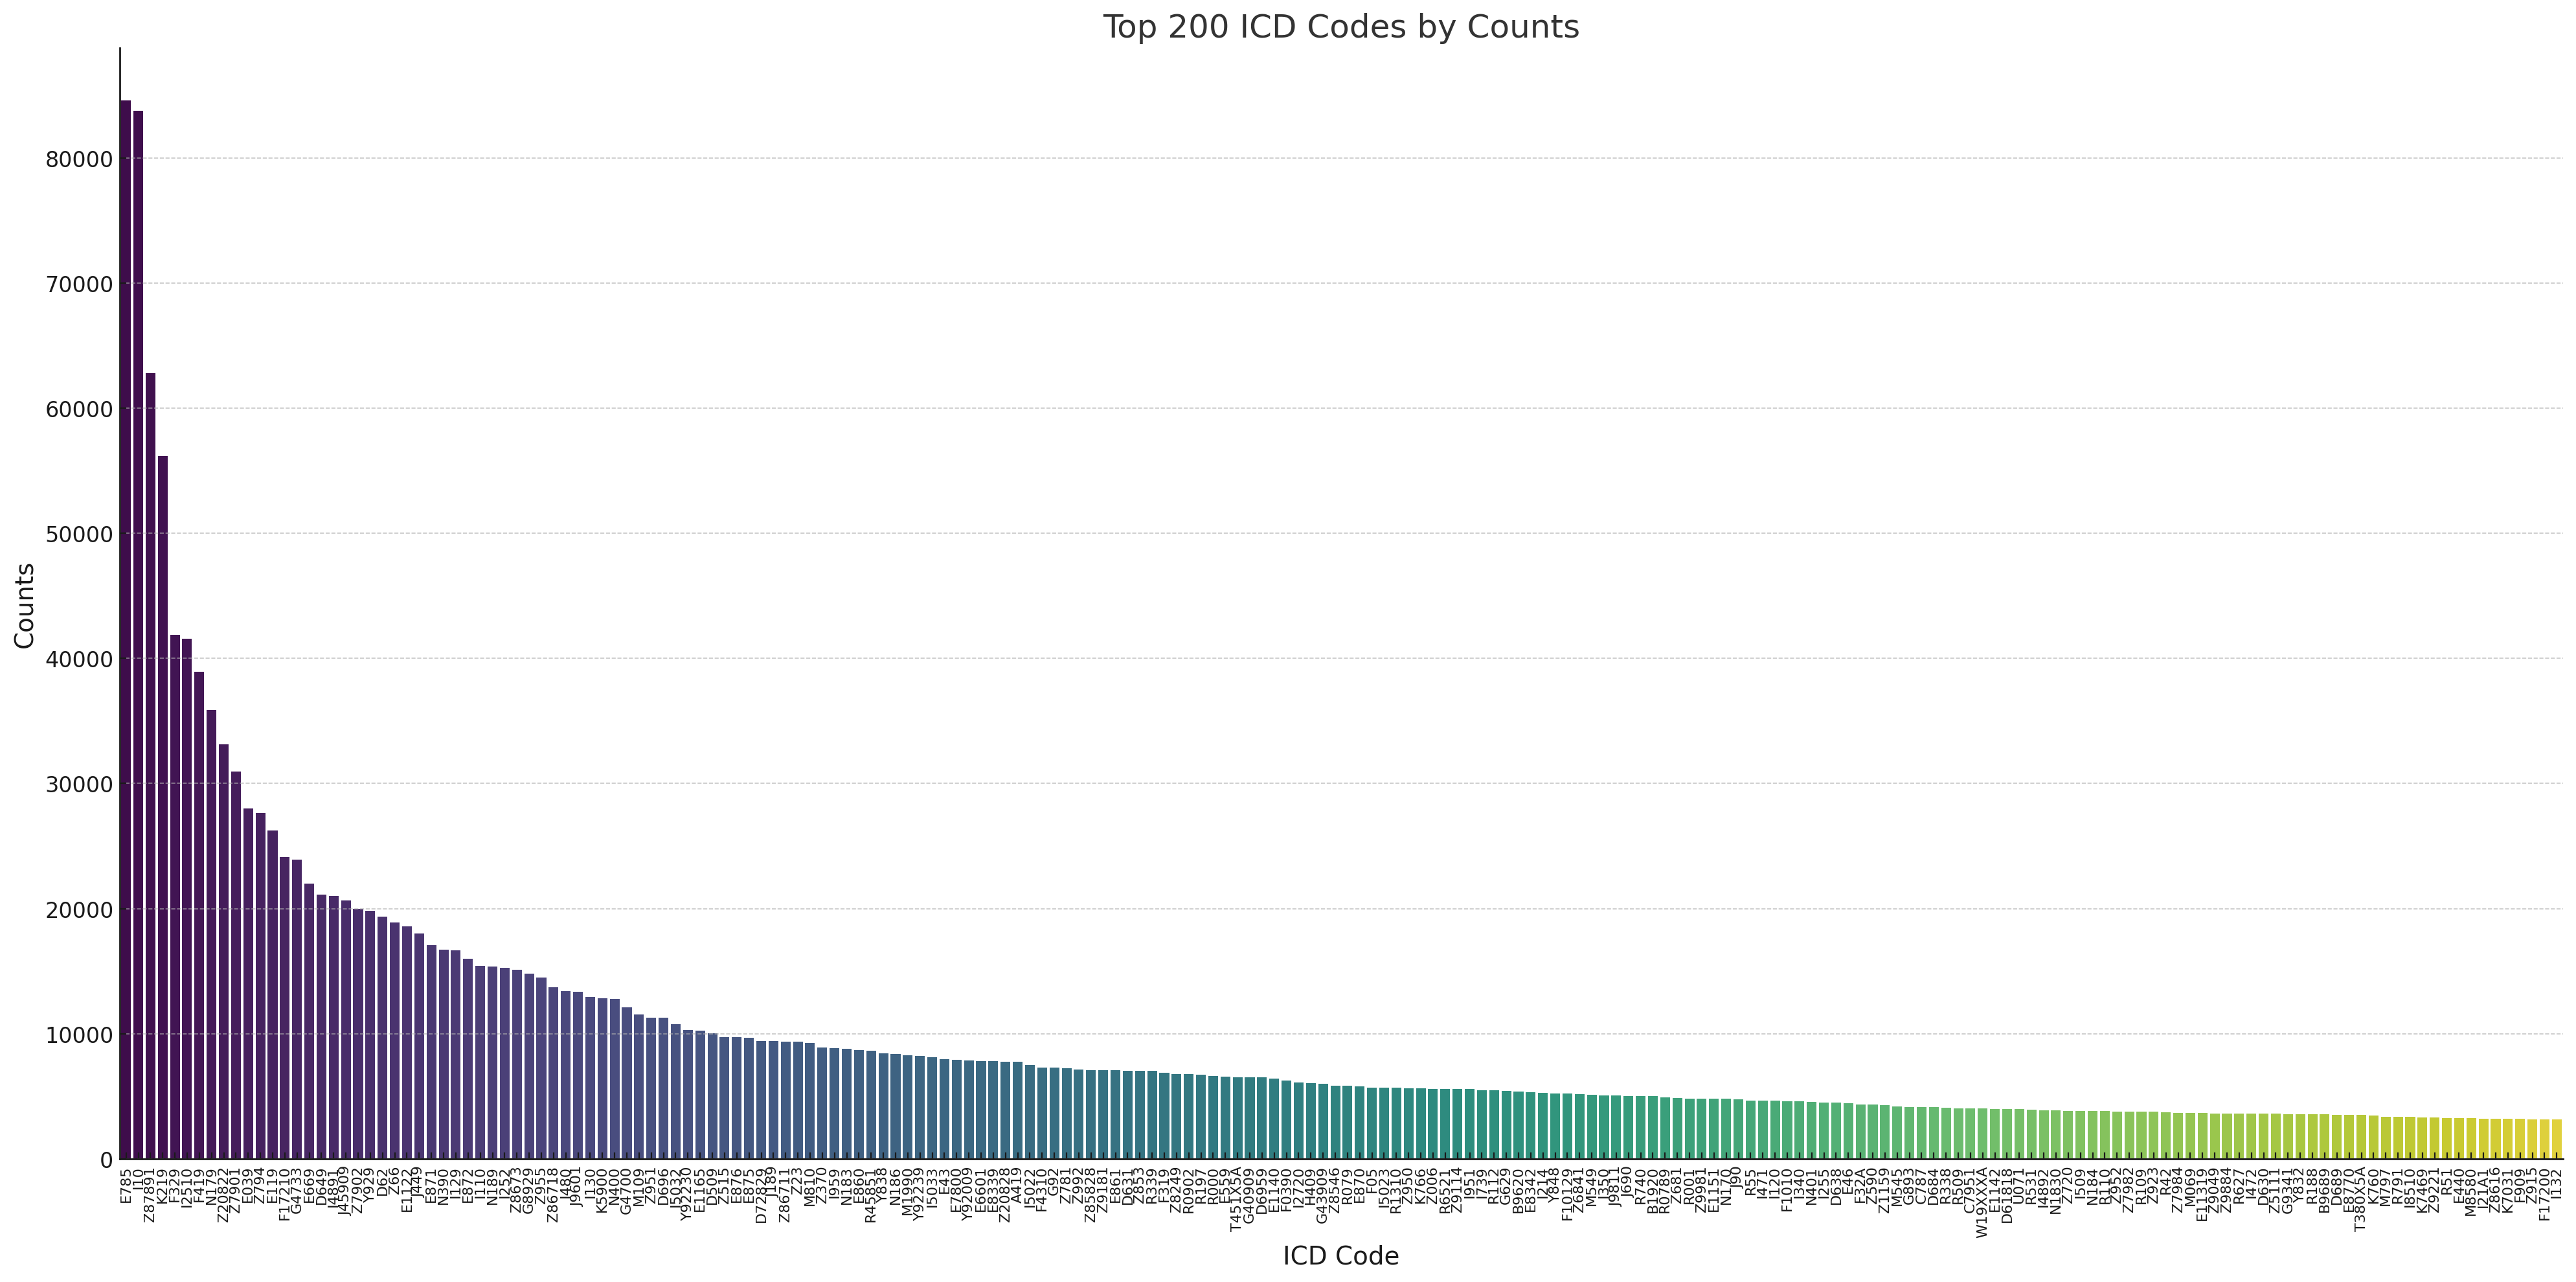
\includegraphics[width=0.8\textwidth]{icd_code_distribution.png}
    \caption{Distribution of ICD Code Frequencies in the Dataset}
    \label{fig:icd_distribution}
\end{figure}

\subsection{Data Preprocessing}
\begin{itemize}
    \item \textbf{Text Cleaning}: Removed non-alphabetic characters, converted text to lowercase, and eliminated extra whitespace.
    \item \textbf{Stopword Removal}: Used NLTK's list of English stopwords to remove common words that do not contribute to meaning.
    \item \textbf{Tokenization and Lemmatization}: Split text into individual words and lemmatized them to reduce inflectional forms.
    \item \textbf{Handling Missing Values}: Identified and addressed missing or incomplete data entries to ensure data integrity.
\end{itemize}

\section{Hybrid Data Augmentation}
To address data imbalance, we implemented a hybrid data augmentation strategy:

\subsection{Retrieval Augmented Generation (RAG)}
\begin{itemize}
    \item \textbf{Concept}: RAG combines retrieval mechanisms with generative models to produce contextually relevant synthetic data.
    \item \textbf{Implementation}: Explored RAG pipelines with local Language Models (LLMs) using tools like \textbf{LangChain} and \textbf{Ollama}.
    \item \textbf{Knowledge Bases}: Connected RAG to medical knowledge graphs and ontologies to retrieve detailed descriptions and generate realistic synthetic clinical notes for rare ICD codes.
    \item \textbf{Integration with Ontologies}: Retrieved relevant medical concepts from ontologies and used them as prompts for the generative model to ensure medical accuracy.
\end{itemize}

\subsection{Ontology-Based Techniques}
\begin{itemize}
    \item \textbf{Knowledge Graphs}: Downloaded and integrated publicly available medical knowledge graphs, including \textbf{SNOMED CT}, \textbf{RxNorm}, \textbf{UMLS}, and others.
    \item \textbf{Entity Incorporation}: Ensured that synthetic notes incorporate medically accurate entities from these ontologies.
    \item \textbf{Semantic Consistency}: Maintained semantic consistency by aligning generated notes with the hierarchical structure of medical concepts.
\end{itemize}

\section{Transformer-Based Model Development}

\subsection{Justification for Model Choice}
Transformer-based models are adept at capturing long-range dependencies and contextual information, which is essential for processing lengthy clinical narratives. Models like \textbf{ClinicalBERT} are pre-trained on biomedical texts, offering domain-specific language understanding. \textbf{Longformer} is designed to handle longer sequences efficiently, making it suitable for processing entire clinical notes without truncation.

\subsection{Model Implementation}
\begin{itemize}
    \item \textbf{ClinicalBERT}: Fine-tuned on our dataset to capture domain-specific language patterns.
    \item \textbf{Longformer}: Employed for its extended context window, allowing the model to process full-length clinical documents.
    \item \textbf{Embedding Generation}: Generated contextual embeddings for clinical notes and ICD code descriptions.
    \item \textbf{Mapping Mechanism}: Designed a mechanism to map clinical note embeddings to ICD code embeddings using similarity measures or learned projections.
\end{itemize}

\subsection{Challenges and Solutions}
\begin{itemize}
    \item \textbf{Computational Complexity}: Addressed the high computational cost of processing long sequences by optimizing batch sizes and leveraging efficient transformer architectures.
    \item \textbf{Handling Rare Codes}: Incorporated techniques like focal loss to focus learning on less frequent codes.
\end{itemize}

\section{Knowledge Integration}
\begin{itemize}
    \item \textbf{Ontology Mapping}: Mapped clinical entities extracted from notes to corresponding concepts in medical ontologies.
    \item \textbf{Knowledge Graph Embeddings}: Incorporated knowledge graph embeddings to enrich model understanding of medical concepts and relationships.
    \item \textbf{Semantic Enrichment}: Augmented input representations with ontology-based features to provide additional context to the model.
\end{itemize}

\section{Multi-Label Classification Techniques}
To handle the extensive label space and hierarchical nature of ICD codes:

\begin{itemize}
    \item \textbf{Label Embedding}: Represented ICD codes in a continuous embedding space to capture semantic relationships, using methods like Word2Vec or GloVe trained on medical corpora.
    \item \textbf{Hierarchical Classification}: Utilized the hierarchical structure of ICD codes to inform the classification process, implementing tree-based models that predict codes at different levels.
    \item \textbf{Label Grouping}: Grouped similar ICD codes based on semantic similarity or clinical relevance to reduce complexity and improve model efficiency.
    \item \textbf{Curriculum Learning}: Applied curriculum learning strategies to train the model progressively, starting with higher-level codes and moving to more specific ones.
\end{itemize}

\section{Model Training and Evaluation}
\begin{itemize}
    \item \textbf{Loss Functions}: Implemented \textbf{Focal Loss} to focus learning on hard-to-classify and rare codes.
    \item \textbf{Sampling Techniques}: Employed oversampling of rare classes and undersampling of frequent classes to balance the training data.
    \item \textbf{Evaluation Metrics}: Used metrics like \textbf{Macro F1-Score} and \textbf{F2-Score} to evaluate performance, especially on rare codes.
    \item \textbf{Cross-Validation}: Performed stratified k-fold cross-validation to ensure robustness of results.
\end{itemize}

\section{Explainability Integration}
\begin{itemize}
    \item \textbf{Techniques Used}: Integrated explainability methods such as \textbf{SHAP}, \textbf{LIME}, and \textbf{Integrated Gradients}.
    \item \textbf{Rationale for Choice}:
    \begin{itemize}
        \item \textbf{SHAP}: Provides global and local explanations, showing feature importance.
        \item \textbf{LIME}: Offers local interpretability by approximating the model locally with interpretable models.
        \item \textbf{Integrated Gradients}: Attributes the prediction to input features by accumulating gradients.
    \end{itemize}
    \item \textbf{Visualization}: Developed visualizations to present explanations to clinicians, enhancing transparency and trust.
    \item \textbf{Clinician Feedback}: Collaborated with healthcare professionals to validate the usefulness of the explanations provided.
\end{itemize}

\section{Similarity Matching Using MinHash}
As part of data exploration and preprocessing:

\subsection{Objective}
Identify duplicate or highly similar clinical notes to reduce redundancy and improve data quality.

\subsection{Methodology}
\begin{itemize}
    \item \textbf{Text Preprocessing}: Preprocessed clinical notes to remove noise and standardize text.
    \item \textbf{MinHash and LSH}: Used \textbf{MinHash} and \textbf{Locality Sensitive Hashing (LSH)} to compute similarity between documents.
    \item \textbf{Threshold Setting}: Set a threshold (e.g., 90\% similarity) to identify similar pairs.
\end{itemize}

\subsection{Results}
\begin{itemize}
    \item Identified 260 notes with over 90\% similarity.
    \item Found six notes with over 97\% similarity, indicating nearly identical content.
\end{itemize}

\subsection{Verification}
Consulted with medical experts to confirm the validity of identified similarities.

\subsection{Implications}
\begin{itemize}
    \item Reducing redundancy in the dataset.
    \item Potentially improving model training by eliminating duplicate information.
\end{itemize}

\section{Implementation Details}
\begin{itemize}
    \item \textbf{Libraries and Tools}:
    \begin{itemize}
        \item \textbf{Python}: Programming language for model development.
        \item \textbf{Pandas, NumPy}: Data manipulation and analysis.
        \item \textbf{DuckDB}: In-memory database for data storage and querying.
        \item \textbf{NLTK, SpaCy}: Natural language processing tasks.
        \item \textbf{Scikit-learn}: Machine learning algorithms and evaluation metrics.
        \item \textbf{PyTorch, Hugging Face Transformers}: Deep learning frameworks for model implementation.
    \end{itemize}
    \item \textbf{Computational Resources}:
    \begin{itemize}
        \item Upgraded hardware to support intensive computations, including increasing RAM to 64GB and adding a 4TB SSD.
        \item Utilized GPU acceleration where available to speed up model training.
    \end{itemize}
    \item \textbf{Data Handling}:
    \begin{itemize}
        \item Ensured compliance with data privacy regulations by securely handling patient data and anonymizing information where necessary.
        \item Implemented secure data storage and access protocols to protect sensitive information.
    \end{itemize}
\end{itemize}

\section{Flow Diagram}
\begin{figure}[H]
    \centering
    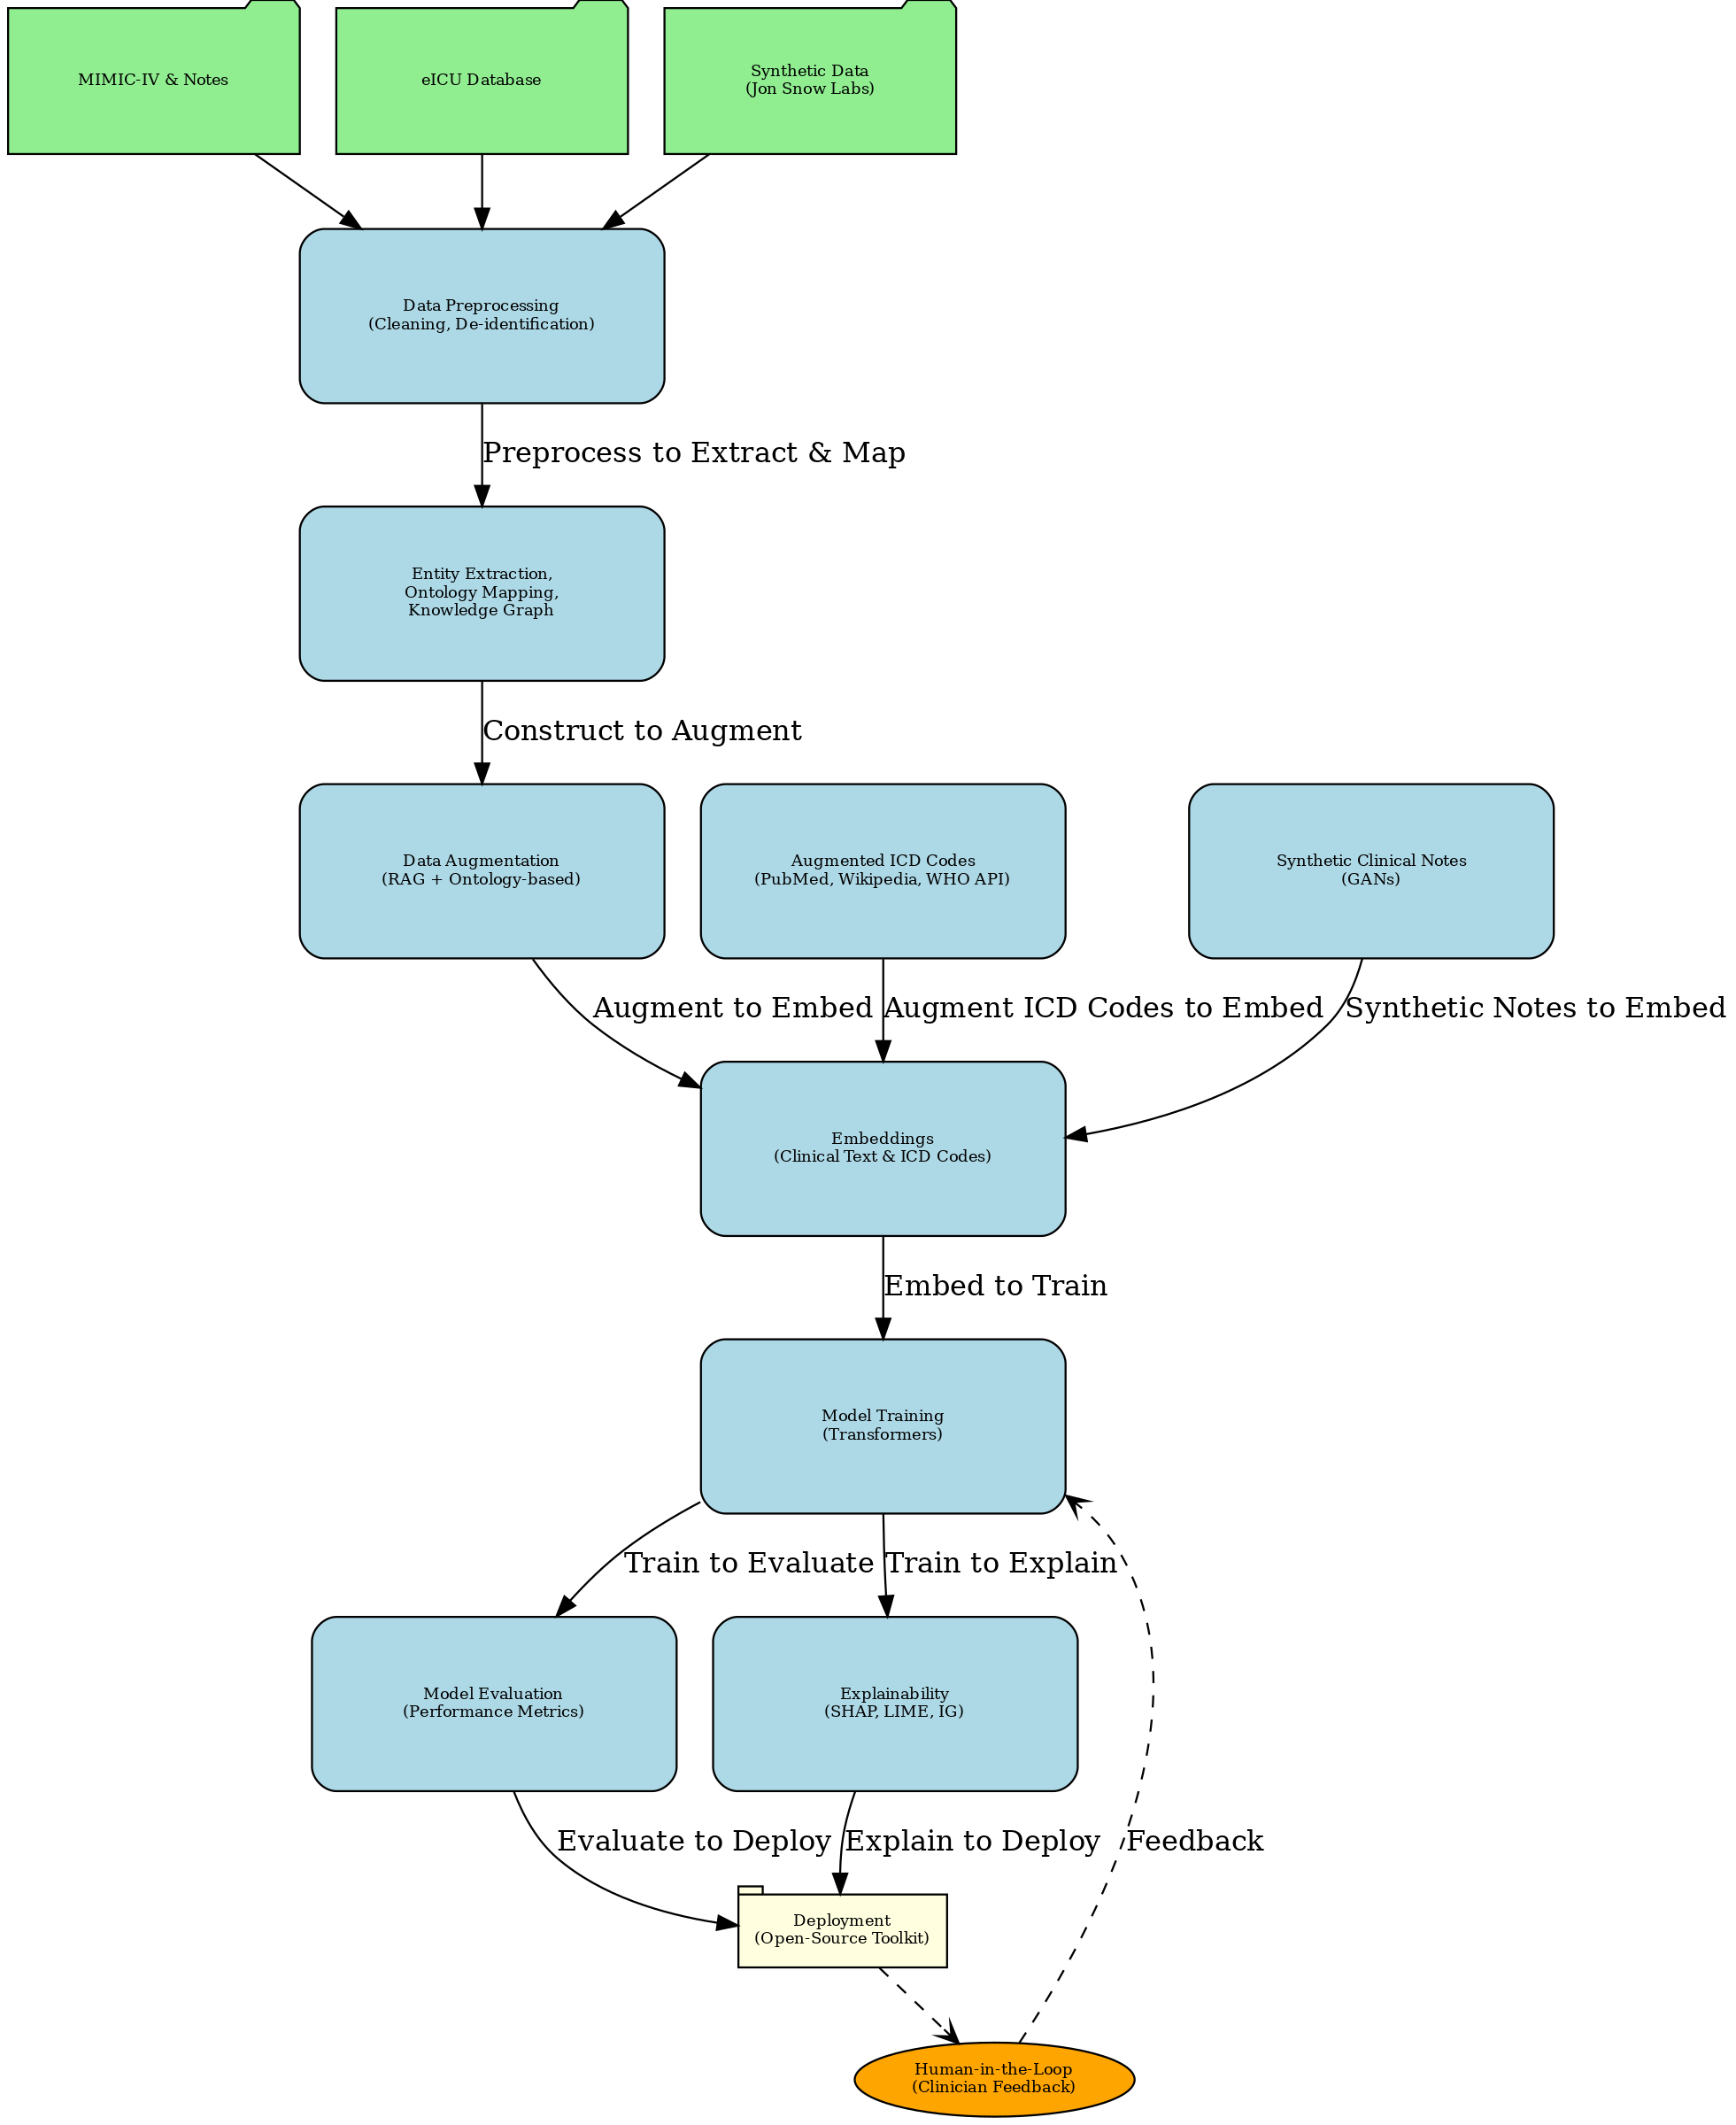
\includegraphics[width=\textwidth]{methodology_flow_diagram.png}
    \caption{Flow Diagram of the Proposed Methodology}
\end{figure}

\chapter{Dataset Understanding}

\section{MIMIC-IV Clinical Database}

\subsection{Overview}
\begin{itemize}
    \item \textbf{Description}: The Medical Information Mart for Intensive Care IV (MIMIC-IV) is a large, publicly available database comprising de-identified health-related data associated with patients who stayed in critical care units of the Beth Israel Deaconess Medical Center~\cite{johnson2016mimic}.
    \item \textbf{Components}:
    \begin{itemize}
        \item \textbf{Clinical Data}: Contains detailed information on patient demographics, vital signs, laboratory tests, medications, and procedures.
        \item \textbf{Notes}: Includes unstructured clinical notes such as discharge summaries, radiology reports, and physician notes.
    \end{itemize}
\end{itemize}

\subsection{Data Characteristics}
\begin{itemize}
    \item \textbf{Patient Population}: Over 40,000 patients, providing a diverse dataset.
    \item \textbf{Clinical Notes}:
    \begin{itemize}
        \item Approximately 330,000 unique clinical notes.
        \item Focus on \textbf{discharge summaries}, which are comprehensive documents summarizing a patient's hospital stay.
        \item Average length of discharge summaries: 1,500 words.
    \end{itemize}
    \item \textbf{ICD Codes}:
    \begin{itemize}
        \item Linked to patient admissions via \texttt{hadm\_id} and \texttt{subject\_id}.
        \item Exhibits a long-tailed distribution, with a small number of codes appearing frequently and many codes being rare.
        \item Total unique ICD codes in database: Approximately 19980. (ICD 10 CM codes are around 70000)
    \end{itemize}
\end{itemize}

\section{Data Preprocessing}

\subsection{Text Preprocessing}
\begin{itemize}
    \item \textbf{Cleaning}: Removed protected health information (PHI) placeholders and irrelevant content.
    \item \textbf{Normalization}: Standardized abbreviations and expanded shorthand notations using medical dictionaries.
    \item \textbf{Segmentation}: Divided notes into sections (e.g., History of Present Illness, Medications) to capture structured information.
\end{itemize}

\subsection{Handling Imbalanced Data}
\begin{itemize}
    \item \textbf{Analysis}: Identified that certain ICD codes dominate the dataset, leading to imbalance.
    \item \textbf{Visualization}: Created histograms and cumulative distribution plots to visualize code frequency distribution (Figure~\ref{fig:icd_distribution}).
    \item \textbf{Approach}: Planned to use data augmentation techniques to generate synthetic data for rare codes.
\end{itemize}

% \begin{figure}[H]
%     \centering
%     \includegraphics[width=0.8\textwidth]{code_frequency_distribution.png}
%     \caption{ICD Code Frequency Distribution}
%     \label{fig:code_frequency}
% \end{figure}

\section{Knowledge Graphs and Ontologies}

\subsection{Resources Utilized}
\begin{itemize}
    \item \textbf{SNOMED CT}: A comprehensive clinical terminology covering diseases, findings, procedures, and more.
    \item \textbf{RxNorm}: Provides normalized names for clinical drugs and links to many drug vocabularies.
    \item \textbf{UMLS Metathesaurus}: Integrates various biomedical vocabularies and standards.
    \item \textbf{OMOP Vocabulary}: Standardized vocabularies used in observational health data.
\end{itemize}

\subsection{Integration}
\begin{itemize}
    \item \textbf{Purpose}: Enrich clinical notes with structured medical knowledge.
    \item \textbf{Method}: Map extracted entities from clinical notes to corresponding concepts in these ontologies using entity recognition and linking algorithms.
    \item \textbf{Challenges}: Addressed issues with synonymy and polysemy by leveraging context-aware mapping techniques.
\end{itemize}

\section{Other Datasets and Resources}

\subsection{Additional Resources}
\begin{itemize}
    \item \textbf{eICU Collaborative Research Database}: Contains data from intensive care units, providing critical patient information.
    \item \textbf{Drug Repurposing Knowledge Graph (DRKG)}: A comprehensive biological knowledge graph relating genes, compounds, diseases, etc.
    \item \textbf{Clinical Trials Knowledge Graph (CTKG)}: A knowledge graph constructed over clinical trial data.
    \item \textbf{Embeddings Repository}: Contains pre-trained embeddings of medical concepts.
    \item \textbf{Health Knowledge Graph}: Supplementary material containing health-related knowledge.
\end{itemize}

\section{Data Storage and Management}

\subsection{Data Volume}
\begin{itemize}
    \item \textbf{Challenge}: Handling large datasets necessitated efficient storage solutions.
    \item \textbf{Solution}: Chose DuckDB for its ability to process large datasets in-memory using SQL.
\end{itemize}

\subsection{Data Access}
\begin{itemize}
    \item \textbf{Efficiency}: Facilitated quick querying and data manipulation for exploration and preprocessing.
    \item \textbf{Scalability}: Supported scaling up as more data was integrated into the project.
\end{itemize}

\section{Data Security and Compliance}

\subsection{Ethical Considerations}
\begin{itemize}
    \item \textbf{Data Privacy}: Ensured adherence to data use agreements and ethical guidelines.
    \item \textbf{Anonymization}: Worked with de-identified data to protect patient privacy.
    \item \textbf{Access Control}: Implemented secure access protocols for sensitive datasets.
    \item \textbf{Compliance}: Complied with regulations such as HIPAA for handling medical data.
\end{itemize}

\chapter{Results}

\section{Baseline Model Experiments}

\subsection{K-Nearest Neighbors (KNN) Classifier}
\begin{itemize}
    \item \textbf{Objective}: Establish a baseline for multi-label ICD code prediction using simple models.
    \item \textbf{Methodology}:
    \begin{itemize}
        \item \textbf{Text Vectorization}: Used TF-IDF vectorizer with a maximum of 5,000 features and n-gram range of (1,2).
        \item \textbf{Multi-Label Binarization}: Applied \textbf{MultiLabelBinarizer} to handle multiple ICD codes per clinical note.
        \item \textbf{Model Training}: Trained a KNN classifier on the vectorized text data.
    \end{itemize}
    \item \textbf{Results}:
    \begin{itemize}
        \item \textbf{Evaluation Metrics}: Used Hamming Loss and Macro F1-Score to assess performance.
        \item \textbf{Performance}: The model achieved a Macro F1-Score of 0.12, indicating poor performance, especially on rare codes.
        \item \textbf{Analysis}: High Hamming Loss and low F1-Score confirmed that the model struggled with data imbalance and text complexity.
    \end{itemize}
\end{itemize}

\subsection{Observations}
\begin{itemize}
    \item The baseline model highlighted the challenges in predicting ICD codes using traditional machine learning approaches.
    \item Reinforced the need for advanced models that can handle complex clinical texts and data imbalance.
\end{itemize}

\section{Similarity Matching Using MinHash}

\subsection{Objective}
Identify duplicate or highly similar clinical notes to reduce redundancy and potentially improve model training.

\subsection{Methodology}
\begin{itemize}
    \item \textbf{Text Preprocessing}: Applied standard preprocessing steps to clean the text.
    \item \textbf{MinHash and LSH}: Used MinHash to create signatures for each document and Locality Sensitive Hashing (LSH) to efficiently identify similar documents.
    \item \textbf{Threshold Setting}: Set similarity thresholds (e.g., 90\% and 97\%) to identify pairs of similar notes.
\end{itemize}

\subsection{Results}
\begin{itemize}
    \item Identified 260 notes with over 90\% similarity.
    \item Found six notes with over 97\% similarity, indicating nearly identical content.
    \item Verification with a medical expert confirmed that these notes were indeed similar or duplicates.
\end{itemize}

\subsection{Implications}
\begin{itemize}
    \item Removing or consolidating similar notes can reduce data redundancy.
    \item May improve model performance by preventing the model from being biased towards duplicated information.
\end{itemize}

\section{Challenges Identified}
\begin{itemize}
    \item \textbf{Data Imbalance}: The initial models confirmed that frequent codes dominate predictions, and rare codes are often missed.
    \item \textbf{Model Limitations}: Simple models like KNN are insufficient for capturing the complexity of clinical narratives.
    \item \textbf{Need for Advanced Techniques}: Emphasized the importance of implementing transformer-based models and data augmentation strategies.
\end{itemize}

\chapter{Conclusion and Work Timeline}

\section{Summary of Work}
In the initial phase of this project, we have:
\begin{itemize}
    \item Established a robust development environment with appropriate tools and infrastructure.
    \item Explored and acquired various datasets and medical knowledge graphs to support data augmentation and knowledge integration.
    \item Conducted data exploration and preprocessing, including identifying redundant clinical notes.
    \item Implemented baseline models to understand the challenges in predicting ICD codes.
    \item Identified key challenges such as data imbalance, complexity of clinical texts, and the limitations of traditional machine learning models.
\end{itemize}

\section{Future Work}
Moving forward, the following tasks are planned:

\subsection{Phase 1: Data Augmentation (Months 3-5)}
\begin{itemize}
    \item Implement hybrid data augmentation techniques combining RAG and ontology-based methods.
    \item Generate synthetic clinical notes for rare ICD codes to balance the dataset.
    \item Validate the quality of synthetic data with clinical experts.
\end{itemize}

\subsection{Phase 2: Transformer-Based Model Development (Months 5-7)}
\begin{itemize}
    \item Develop and fine-tune transformer-based models suitable for long clinical documents.
    \item Integrate knowledge graph embeddings to enhance the model's understanding of medical concepts and relationships.
    \item Address computational challenges by optimizing model architectures and training procedures.
\end{itemize}

\subsection{Phase 3: Model Training and Evaluation (Months 7-8)}
\begin{itemize}
    \item Train the model using the augmented dataset.
    \item Evaluate performance using appropriate metrics, focusing on rare code prediction.
    \item Perform error analysis to identify areas for improvement.
\end{itemize}

\subsection{Phase 4: Explainability Integration (Months 8-9)}
\begin{itemize}
    \item Integrate explainability techniques to provide interpretable predictions.
    \item Develop visualization tools for presenting explanations to clinicians.
    \item Gather feedback from healthcare professionals to refine explanations.
\end{itemize}

\subsection{Phase 5: Deployment and Validation (Months 9-10)}
\begin{itemize}
    \item Deploy the model as an open-source toolkit.
    \item Validate the model with clinician feedback and refine as necessary.
    \item Document the methodology and results for publication.
\end{itemize}

\section{Timeline}
\begin{figure}[H]
    \centering
    \begin{ganttchart}[
        hgrid,
        vgrid,
        x unit=0.7cm,
        y unit title=0.6cm,
        y unit chart=0.6cm,
        title height=1,
        bar/.style={fill=blue!50},
        bar height=0.5
    ]{1}{11}
        \gantttitle{Project Timeline (Months)}{11} \\
        \gantttitlelist{1,...,11}{1} \\
        \ganttbar{Phase 1: Data Augmentation}{3}{5} \\
        \ganttbar{Phase 2: Model Development}{5}{7} \\
        \ganttbar{Phase 3: Training and Evaluation}{7}{8} \\
        \ganttbar{Phase 4: Explainability Integration}{8}{9} \\
        \ganttbar{Phase 5: Deployment \& Validation}{9}{10} \\
    \end{ganttchart}
    \caption{Gantt Chart of Planned Work Timeline}
\end{figure}

\section{Potential Challenges and Contingency Plans}
\begin{itemize}
    \item \textbf{Computational Resources}: If computational limitations arise, we will explore cloud-based solutions or optimize model architectures for efficiency.
    \item \textbf{Data Quality}: In case synthetic data does not sufficiently improve model performance, we will consider alternative data augmentation techniques or focus on enhancing model robustness.
    \item \textbf{Model Interpretability}: If explainability methods do not meet clinician requirements, we will investigate other interpretability frameworks or simplify the model for better transparency.
\end{itemize}

\section{Concluding Remarks}
This thesis aims to contribute to the field of automated ICD coding by addressing critical challenges through innovative methods. By combining hybrid data augmentation, advanced modeling techniques, and explainability, we anticipate improving prediction accuracy, particularly for rare ICD codes, and enhancing the usability of automated coding systems in clinical settings. The successful completion of this project could pave the way for further applications of data augmentation and knowledge integration in medical NLP tasks.

% Bibliography
\begin{thebibliography}{99}

\bibitem{who2019icd11}
World Health Organization. \textit{International Classification of Diseases 11th Revision (ICD-11)}. (2019).

\bibitem{dong2022automated}
Dong, H., Suárez-Paniagua, V., Whiteley, W., \& Wu, H. Automated clinical coding: what, why, and where we are? \textit{npj Digital Medicine} \textbf{5}, 159 (2022).

\bibitem{edin2023automated}
Edin, J., Jensen, S.M., Sahlgren, M., Lövgren, J., \& Henriksson, A. Automated medical coding on MIMIC-III and MIMIC-IV: a critical review and replicability study. In \textit{Proceedings of the 46th International ACM SIGIR Conference on Research and Development in Information Retrieval}, 2023.

\bibitem{farkas2008automatic}
Farkas, R. \& Szarvas, G. Automatic construction of rule-based ICD-9-CM coding systems. \textit{BMC Bioinformatics} \textbf{9}, 1–9 (2008).

\bibitem{scheurwegs2017data}
Scheurwegs, E. et al. Data integration of structured and unstructured sources for assigning clinical codes to patient stays. \textit{Journal of the American Medical Informatics Association} \textbf{24}, e68–e76 (2017).

\bibitem{perotte2014diagnosis}
Perotte, A. et al. Diagnosis code assignment: models and evaluation metrics. \textit{Journal of the American Medical Informatics Association} \textbf{21}, 231–237 (2014).

\bibitem{lecun2015deep}
LeCun, Y., Bengio, Y., \& Hinton, G. Deep learning. \textit{Nature} \textbf{521}, 436–444 (2015).

\bibitem{kim2014convolutional}
Kim, Y. Convolutional neural networks for sentence classification. In \textit{Proceedings of the 2014 Conference on Empirical Methods in Natural Language Processing (EMNLP)}, 1746–1751 (2014).

\bibitem{mullenbach2018explainable}
Mullenbach, J., Wiegreffe, S., Duke, J., Sun, J., \& Eisenstein, J. Explainable prediction of medical codes from clinical text. In \textit{Proceedings of the 2018 Conference of the North American Chapter of the Association for Computational Linguistics}, 1101–1111 (2018).

\bibitem{li2020multi}
Li, F. \& Yu, H. ICD coding from clinical text using multi-filter residual convolutional neural network. In \textit{Proceedings of the AAAI Conference on Artificial Intelligence}, vol. 34, 8180–8187 (2020).

\bibitem{hochreiter1997long}
Hochreiter, S. \& Schmidhuber, J. Long short-term memory. \textit{Neural Computation} \textbf{9}, 1735–1780 (1997).

\bibitem{vu2020label}
Vu, T., Nguyen, D. Q., \& Nguyen, A. A label attention model for ICD coding from clinical text. \textit{Journal of Biomedical Informatics} \textbf{102}, 103381 (2020).

\bibitem{devlin2019bert}
Devlin, J., Chang, M.-W., Lee, K., \& Toutanova, K. BERT: Pre-training of deep bidirectional transformers for language understanding. In \textit{Proceedings of NAACL-HLT}, 4171–4186 (2019).

\bibitem{gao2021limitations}
Gao, S. et al. Limitations of transformers on clinical text classification. \textit{IEEE Journal of Biomedical and Health Informatics} \textbf{25}, 3596–3607 (2021).

\bibitem{huang2022plm}
Huang, C.-W., Tsai, S.-C., \& Chen, Y.-N. PLM-ICD: Automatic ICD coding with pre-trained language models. In \textit{Proceedings of the 4th Clinical Natural Language Processing Workshop}, 10–20 (2022).

\bibitem{heo2022medical}
Heo, T.-S., Jo, B., Yoo, Y., Lee, K., Park, Y., \& Kim, K. Medical code prediction from discharge summary: Document to sequence BERT using sequence attention. In \textit{2022 International Conference on Electronics, Information, and Communication (ICEIC)}, 1–4 (2022).

\bibitem{bengio2009curriculum}
Bengio, Y., Louradour, J., Collobert, R., \& Weston, J. Curriculum learning. In \textit{Proceedings of the 26th Annual International Conference on Machine Learning}, 41–48 (2009).

\bibitem{ren2022hicu}
Ren, W., Zeng, R., Wu, T., Zhu, T., \& Krishnan, R. G. HiCu: Leveraging hierarchy for curriculum learning in automated ICD coding. In \textit{Proceedings of the Machine Learning for Healthcare Conference}, 1–24 (2022).

\bibitem{johnson2016mimic}
Johnson, A. E. W. et al. MIMIC-III, a freely accessible critical care database. \textit{Scientific Data} \textbf{3}, 160035 (2016).

\bibitem{rios2018few}
Rios, A. \& Kavuluru, R. Few-shot and zero-shot multi-label learning for structured label spaces. In \textit{Proceedings of the 2018 Conference on Empirical Methods in Natural Language Processing}, 3132–3142 (2018).

\bibitem{wrenn2010quantifying}
Wrenn, J. O., Stein, D. M., Bakken, S., \& Stetson, P. D. Quantifying clinical narrative redundancy in an electronic health record. \textit{Journal of the American Medical Informatics Association} \textbf{17}, 49–53 (2010).

\bibitem{holzinger2017we}
Holzinger, A. et al. What do we need to build explainable AI systems for the medical domain? \textit{arXiv preprint arXiv:1712.09923} (2017).

\bibitem{edin2024unsupervised}
Edin, J., Borgholt, L., Maistro, M., Havtorn, J. D., Maaløe, L., \& Ruotsalo, T. An unsupervised approach to achieve supervised-level explainability in healthcare records. \textit{arXiv preprint arXiv:2406.08958} (2024).

\bibitem{teng2020explainable}
Teng, F., Yang, W., Chen, L., Huang, L., \& Xu, Q. Explainable prediction of medical codes with knowledge graphs. \textit{Frontiers in Bioengineering and Biotechnology} \textbf{8}, 867 (2020).

\bibitem{xie2019ehr}
Xie, X., Xiong, Y., Yu, P. S., \& Zhu, Y. EHR coding with multi-scale feature attention and structured knowledge graph propagation. In \textit{Proceedings of the 28th ACM International Conference on Information and Knowledge Management}, 649–658 (2019).

\bibitem{nickel2017poincare}
Nickel, M. \& Kiela, D. Poincaré embeddings for learning hierarchical representations. In \textit{Advances in Neural Information Processing Systems}, 6338–6347 (2017).

\bibitem{kumichev2024medsyn}
Kumichev, G., Blinov, P., Kuzkina, Y., Goncharov, V., Zubkova, G., Zenovkin, N., Goncharov, A., \& Savchenko, A. MedSyn: LLM-based synthetic medical text generation framework. \textit{arXiv preprint arXiv:2408.02056} (2024).

\bibitem{excoffier2024generalist}
Excoffier, J.-B., Roehr, T., Figueroa, A., Papaioannou, J.-M., Bressem, K., \& Ortala, M. Generalist embedding models are better at short-context clinical semantic search than specialized embedding models. \textit{arXiv preprint arXiv:2401.01943} (2024).

\bibitem{campbell2020computer}
Campbell, S. \& Giadresco, K. Computer-assisted clinical coding: A narrative review of the literature on its benefits, limitations, implementation, and impact on clinical coding professionals. \textit{Health Information Management Journal} \textbf{49}, 5–18 (2020).

\bibitem{kraljevic2021multi}
Kraljevic, Z. et al. Multi-domain clinical natural language processing with MedCAT: The medical concept annotation toolkit. \textit{Artificial Intelligence in Medicine} \textbf{117}, 102083 (2021).

\bibitem{gaebel2020changes}
Gaebel, W., Stricker, J., \& Kerst, A. Changes from ICD-10 to ICD-11 and future directions in psychiatric classification. \textit{Dialogues in Clinical Neuroscience} \textbf{22}, 7–15 (2020).

\bibitem{wang2021meta}
Wang, R. et al. Meta-LMTC: Meta-learning for large-scale multi-label text classification. In \textit{Proceedings of the 2021 Conference on Empirical Methods in Natural Language Processing}, 8633–8646 (2021).

\bibitem{nguyen2023mimic}
Nguyen, T.-T., Schlegel, V., Kashyap, A., Winkler, S., Huang, S.-S., Liu, J.-J., \& Lin, C.-J. MIMIC-IV-ICD: A New Benchmark for Extreme Multi-Label Classification. In \textit{Proceedings of the 61st Annual Meeting of the Association for Computational Linguistics}, 2023.

\end{thebibliography}

\end{document}
